\documentclass[11pt,twocolumn]{article}

% ─── Packages ─────────────────────────────────────────────────────
\usepackage[T1]{fontenc}
\usepackage[utf8]{inputenc}
\usepackage{lmodern}
\usepackage[margin=0.85in,top=1in,bottom=1in]{geometry}
\usepackage{graphicx}
\usepackage{xcolor}
\usepackage{tikz}
\usetikzlibrary{positioning,arrows.meta,fit,shapes.geometric,calc,decorations.pathreplacing,backgrounds}
\usepackage{booktabs}
\usepackage{enumitem}
\usepackage{listings}
\usepackage{hyperref}
\usepackage{amsmath,amssymb}
\usepackage{caption}
\usepackage{subcaption}
\usepackage{fancyhdr}
\usepackage{titlesec}
\usepackage{abstract}
\usepackage{float}

% ─── Colors ───────────────────────────────────────────────────────
\definecolor{qubesblue}{HTML}{3874D8}
\definecolor{qubesorange}{HTML}{E38B28}
\definecolor{qubesgreen}{HTML}{3FB950}
\definecolor{qubespurple}{HTML}{8957E5}
\definecolor{qubesred}{HTML}{DA3633}
\definecolor{codebg}{HTML}{161B22}
\definecolor{codefg}{HTML}{C9D1D9}
\definecolor{codegreen}{HTML}{7EE787}
\definecolor{codeblue}{HTML}{79C0FF}
\definecolor{accentblue}{HTML}{58A6FF}

% ─── Listings ─────────────────────────────────────────────────────
\lstdefinestyle{terminal}{
    backgroundcolor=\color{codebg},
    basicstyle=\ttfamily\scriptsize\color{codefg},
    keywordstyle=\color{codeblue},
    stringstyle=\color{codegreen},
    commentstyle=\color{gray},
    frame=single,
    rulecolor=\color{gray!30},
    breaklines=true,
    columns=fullflexible,
    xleftmargin=4pt,
    xrightmargin=4pt,
    aboveskip=8pt,
    belowskip=8pt,
}

% ─── Hyperref ─────────────────────────────────────────────────────
\hypersetup{
    colorlinks=true,
    linkcolor=qubesblue,
    citecolor=qubesblue,
    urlcolor=accentblue,
}

% ─── Headers ──────────────────────────────────────────────────────
\pagestyle{fancy}
\fancyhf{}
\fancyhead[L]{\small\textit{qubes-claw: Isolated AI Agent Infrastructure}}
\fancyhead[R]{\small\thepage}
\renewcommand{\headrulewidth}{0.4pt}

% ─── Title ────────────────────────────────────────────────────────
\title{%
    \vspace{-1em}%
    \textbf{\Large qubes-claw: Secure, Isolated AI Agent\\Infrastructure on Qubes OS}\\[6pt]
    \large Multi-Provider LLM Orchestration with Xen-Enforced\\VM Isolation and Airgapped Administration%
}

\author{%
    Gabriele Risso\\
    \texttt{gabri.risso@gmail.com}\\
    \url{https://github.com/GabrieleRisso/qubes-claw}
}

\date{February 2026}

% ══════════════════════════════════════════════════════════════════
\begin{document}
\maketitle
\thispagestyle{fancy}

% ─── Abstract ─────────────────────────────────────────────────────
\begin{abstract}
\noindent
Large Language Model (LLM) agents increasingly require access to sensitive
resources---shells, file systems, APIs, and credentials---creating an expanding
attack surface that traditional sandboxing cannot adequately contain. We present
\textbf{qubes-claw}, an open-source framework that leverages Qubes OS's
Xen-based VM isolation to run AI agents in dedicated virtual machines while
providing airgapped administration from \texttt{dom0}, the most privileged and
network-less control domain. The system supports multiple LLM providers
(Cursor~Pro, OpenAI, Anthropic, Ollama) through a unified proxy architecture,
uses qrexec tunnels over Xen shared memory rather than TCP/IP networking, and
achieves full reboot persistence with zero manual intervention. We describe the
architecture, threat model, security properties, and demonstrate that the
framework imposes negligible latency overhead ($<$5\,ms per API call) while
providing hardware-enforced isolation guarantees that no container-based
solution can match.

\medskip
\noindent\textbf{Keywords:} LLM agents, VM isolation, Qubes OS, Xen hypervisor,
qrexec, airgapped administration, multi-provider AI
\end{abstract}

% ─── 1. Introduction ─────────────────────────────────────────────
\section{Introduction}
\label{sec:intro}

The rapid adoption of autonomous AI agents in software development workflows
has created a fundamental tension between capability and containment. Modern
LLM agents---such as those powered by GPT-5, Claude~4, or open-weight
models---routinely execute shell commands, modify file systems, make network
requests, and manage credentials on behalf of users~\cite{openai2024agents}.
This operational model grants agents a privilege level comparable to the user
themselves, yet the agents operate on instructions derived from probabilistic
language models that can be manipulated through prompt injection, hallucinate
harmful commands, or exfiltrate data through side channels.

Existing mitigation strategies fall into three categories:
\begin{enumerate}[leftmargin=*,topsep=2pt,itemsep=1pt]
    \item \textbf{Process-level sandboxing} (Docker, gVisor, Firecracker):
          Provides namespace isolation but shares the host kernel, leaving a
          large attack surface for privilege escalation.
    \item \textbf{Policy-based access control} (SELinux, AppArmor): Adds
          mandatory access control but cannot prevent data exfiltration through
          legitimate network channels the agent is permitted to use.
    \item \textbf{Air-gapped execution}: Eliminates network vectors but is
          traditionally impractical for agents that require API access to
          cloud-hosted LLMs.
\end{enumerate}

\textbf{qubes-claw} addresses this gap by combining Xen hypervisor-level VM
isolation with a novel qrexec-based tunneling architecture that provides
selective, auditable API access while keeping the administration plane
completely airgapped. The key insight is that \textit{the administration
interface does not need network access}---it only needs structured data flow
from the agent VM, which Xen's shared memory transport (qrexec) provides with
hardware-enforced unidirectional guarantees.

\subsection{Contributions}

\begin{itemize}[leftmargin=*,topsep=2pt,itemsep=1pt]
    \item A \textbf{reference architecture} for running LLM agents in
          Xen-isolated VMs with airgapped administration (Section~\ref{sec:arch}).
    \item A \textbf{multi-provider proxy} supporting Cursor~Pro, OpenAI,
          Anthropic, and Ollama through a single OpenAI-compatible API endpoint
          (Section~\ref{sec:providers}).
    \item A \textbf{qrexec tunnel design} that replaces TCP/IP networking with
          Xen shared memory for dom0-to-VM communication
          (Section~\ref{sec:tunnels}).
    \item A \textbf{defense-in-depth security model} with four enforcement
          layers (Section~\ref{sec:security}).
    \item An \textbf{open-source implementation} with one-command setup scripts
          and full reboot persistence (Section~\ref{sec:impl}).
\end{itemize}

% ─── 2. Background ───────────────────────────────────────────────
\section{Background}
\label{sec:background}

\subsection{Qubes OS and the Xen Security Model}

Qubes OS~\cite{rutkowska2010qubes} implements a security-by-compartmentalization
approach built on the Xen hypervisor. Each security domain runs in a separate
virtual machine (VM), with inter-VM communication mediated exclusively by
\texttt{qrexec}---a custom RPC framework that uses Xen shared memory pages
(\texttt{vchan}) rather than network sockets. The privileged domain
\texttt{dom0} manages all VMs but has \textit{no network interface}, making it
immune to remote exploitation.

\subsection{The Agent Trust Problem}

AI agents operate with delegated authority. When a user instructs an agent to
``refactor the authentication module,'' the agent must read source files,
execute tests, and modify code---actions indistinguishable from an attacker
with shell access. The trust model is:

\begin{equation}
    \mathcal{T}_{\text{agent}} = \mathcal{T}_{\text{user}} - \mathcal{T}_{\text{model}}
\end{equation}

\noindent where $\mathcal{T}_{\text{model}}$ represents the trust deficit from
model unreliability (hallucinations, prompt injection susceptibility, training
data poisoning). Container isolation reduces the blast radius but cannot
eliminate the trust deficit, as the agent typically retains network access to
the LLM API---the same channel that could be used for exfiltration.

% ─── 3. Architecture ─────────────────────────────────────────────
\section{Architecture}
\label{sec:arch}

The qubes-claw architecture separates the system into three trust domains
connected by a minimal, auditable communication channel.

% ─── Architecture Diagram ────────────────────────────────────────
\begin{figure*}[t]
\centering
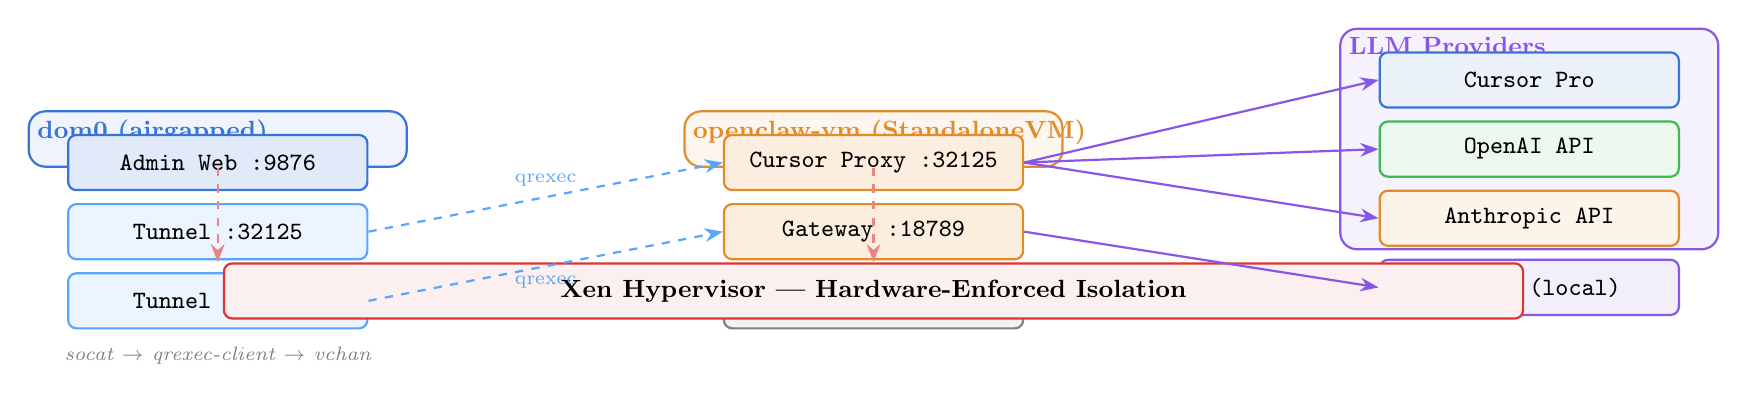
\begin{tikzpicture}[
    >=Stealth,
    node distance=0.6cm,
    box/.style={draw, rounded corners=3pt, minimum width=3.8cm,
                minimum height=0.7cm, font=\small\ttfamily, thick},
    dombox/.style={draw, rounded corners=6pt, thick, inner sep=10pt,
                   minimum width=4.8cm},
    label/.style={font=\small\bfseries, anchor=north west},
    arrow/.style={->, thick, >=Stealth},
    tunnel/.style={->, thick, dashed, >=Stealth, color=accentblue},
]

% dom0
\node[dombox, fill=qubesblue!8, draw=qubesblue] (dom0) at (0,0) {};
\node[label, color=qubesblue] at (dom0.north west) {dom0 (airgapped)};
\node[box, fill=qubesblue!15, draw=qubesblue, below=0.3cm of dom0.north]
    (adminweb) {Admin Web :9876};
\node[box, fill=accentblue!12, draw=accentblue, below=0.15cm of adminweb]
    (tunnel32) {Tunnel :32125};
\node[box, fill=accentblue!12, draw=accentblue, below=0.15cm of tunnel32]
    (tunnel18) {Tunnel :18789};
\node[font=\scriptsize\itshape, color=gray, below=0.1cm of tunnel18]
    (nontcp) {socat $\to$ qrexec-client $\to$ vchan};

% VM
\node[dombox, fill=qubesorange!8, draw=qubesorange, right=3.5cm of dom0] (vm) {};
\node[label, color=qubesorange] at (vm.north west) {openclaw-vm (StandaloneVM)};
\node[box, fill=qubesorange!15, draw=qubesorange, below=0.3cm of vm.north]
    (proxy) {Cursor Proxy :32125};
\node[box, fill=qubesorange!15, draw=qubesorange, below=0.15cm of proxy]
    (gateway) {Gateway :18789};
\node[box, fill=gray!10, draw=gray, below=0.15cm of gateway]
    (connecttcp) {qubes.ConnectTCP};

% Providers
\node[dombox, fill=qubespurple!8, draw=qubespurple, right=3.5cm of vm,
      minimum height=2.8cm] (providers) {};
\node[label, color=qubespurple] at (providers.north west) {LLM Providers};
\node[box, fill=qubesblue!10, draw=qubesblue, below=0.3cm of providers.north]
    (cursor) {Cursor Pro};
\node[box, fill=qubesgreen!10, draw=qubesgreen, below=0.15cm of cursor]
    (openai) {OpenAI API};
\node[box, fill=qubesorange!10, draw=qubesorange, below=0.15cm of openai]
    (anthropic) {Anthropic API};
\node[box, fill=qubespurple!10, draw=qubespurple, below=0.15cm of anthropic]
    (ollama) {Ollama (local)};

% Xen
\node[draw, thick, fill=qubesred!8, draw=qubesred, rounded corners=3pt,
      minimum width=16.5cm, minimum height=0.7cm, font=\small\bfseries,
      below=1.2cm of vm] (xen)
    {Xen Hypervisor --- Hardware-Enforced Isolation};

% Arrows: dom0 -> VM (qrexec tunnels)
\draw[tunnel] (tunnel32.east) -- node[above, font=\scriptsize, color=accentblue]
    {qrexec} (proxy.west);
\draw[tunnel] (tunnel18.east) -- node[below, font=\scriptsize, color=accentblue]
    {qrexec} (gateway.west);

% Arrows: VM -> Providers
\draw[arrow, color=qubespurple] (proxy.east) -- (cursor.west);
\draw[arrow, color=qubespurple] (proxy.east) -- (openai.west);
\draw[arrow, color=qubespurple] (proxy.east) -- (anthropic.west);
\draw[arrow, color=qubespurple] (gateway.east) -- (ollama.west);

% Arrows: everything on Xen
\draw[arrow, color=qubesred!60, dashed] (dom0.south) -- (xen.north -| dom0.south);
\draw[arrow, color=qubesred!60, dashed] (vm.south) -- (xen.north -| vm.south);

\end{tikzpicture}
\caption{qubes-claw system architecture. Dashed blue arrows represent qrexec
tunnels (Xen shared memory). The admin domain \texttt{dom0} has no network
interface; all communication uses \texttt{vchan} pages managed by the
hypervisor. The agent VM connects to LLM providers through standard HTTPS.}
\label{fig:architecture}
\end{figure*}

\subsection{Trust Domains}

\begin{description}[leftmargin=0pt,topsep=4pt,itemsep=2pt]
    \item[dom0 (Administration)] The Qubes control domain. Runs the admin web
        UI, tunnel endpoints, and qrexec policy engine. Has no network stack
        and cannot be compromised remotely. Administers agent VMs through
        structured qrexec calls.
    \item[openclaw-vm (Agent Execution)] A StandaloneVM running the OpenClaw
        proxy, gateway, and AI agents. Has network access to reach LLM
        provider APIs. Isolated from other VMs by the Xen hypervisor.
    \item[LLM Providers (External)] Cloud APIs (OpenAI, Anthropic) or local
        inference (Ollama). The proxy normalizes all providers to an
        OpenAI-compatible API surface.
\end{description}

\subsection{Qrexec Tunnel Design}
\label{sec:tunnels}

The central innovation is replacing TCP/IP networking between dom0 and the
agent VM with qrexec tunnels. Each tunnel consists of:

\begin{enumerate}[leftmargin=*,topsep=2pt,itemsep=1pt]
    \item A \texttt{socat} listener on dom0's localhost (e.g., \texttt{127.0.0.1:32125}).
    \item A \texttt{qrexec-client} invocation that opens a \texttt{vchan}
          connection to the target VM.
    \item A \texttt{qubes.ConnectTCP} handler in the VM that forwards the
          connection to \texttt{localhost:\$PORT} via \texttt{socat}.
\end{enumerate}

\noindent This design has three key properties:

\begin{itemize}[leftmargin=*,topsep=2pt,itemsep=1pt]
    \item \textbf{No network exposure}: dom0 binds only to \texttt{127.0.0.1}.
          The transport layer is Xen shared memory, not TCP/IP.
    \item \textbf{Policy-controlled}: Qrexec policies specify which VMs can
          connect to which services, with tag-based access control.
    \item \textbf{Auditable}: Every qrexec call is logged by the Qubes
          policy engine.
\end{itemize}

\begin{lstlisting}[style=terminal, caption={Dom0 tunnel service template
(\texttt{systemd}). Each tunnel instance binds a local port and forwards
through qrexec.}, label={lst:tunnel}]
# openclaw-tunnel@.service
[Service]
ExecStart=/bin/sh -c "exec socat \
  TCP-LISTEN:%i,bind=127.0.0.1,fork,reuseaddr \
  EXEC:/usr/local/bin/openclaw-tcp-forward %i"
\end{lstlisting}

% ─── 4. Multi-Provider Support ───────────────────────────────────
\section{Multi-Provider Architecture}
\label{sec:providers}

qubes-claw abstracts LLM provider differences behind a unified
OpenAI-compatible API endpoint. The proxy layer translates requests and
normalizes responses, allowing agents to switch providers without
configuration changes.

\begin{table}[h]
\centering
\caption{Supported LLM providers and their characteristics.}
\label{tab:providers}
\small
\begin{tabular}{@{}llll@{}}
\toprule
\textbf{Provider} & \textbf{Auth} & \textbf{Network} & \textbf{Models} \\
\midrule
Cursor Pro & Session & HTTPS & Auto, GPT-5, Claude~4 \\
OpenAI     & API key & HTTPS & GPT-4o, o1, o3-mini \\
Anthropic  & API key & HTTPS & Sonnet~4, Opus~4 \\
Ollama     & None    & Local & Llama~3, Qwen, DeepSeek \\
\bottomrule
\end{tabular}
\end{table}

\noindent The multi-provider configuration in Listing~\ref{lst:config}
demonstrates how providers are declared in \texttt{openclaw.json}. The system
supports simultaneous provider registration with model-level routing.

\begin{lstlisting}[style=terminal, caption={Multi-provider configuration
excerpt. API keys use environment variable placeholders and never appear in
version control.}, label={lst:config}]
{
  "models": {
    "mode": "merge",
    "providers": {
      "cursor":    { "baseUrl": "http://127.0.0.1:32125/v1" },
      "openai":    { "apiKey": "${OPENAI_API_KEY}" },
      "anthropic": { "apiKey": "${ANTHROPIC_API_KEY}" },
      "ollama":    { "baseUrl": "http://127.0.0.1:11434/v1" }
    }
  }
}
\end{lstlisting}

% ─── 5. Security Model ───────────────────────────────────────────
\section{Security Analysis}
\label{sec:security}

qubes-claw implements a defense-in-depth security model with four enforcement
layers, each providing independent containment guarantees.

% ─── Security Diagram ────────────────────────────────────────────
\begin{figure}[h]
\centering
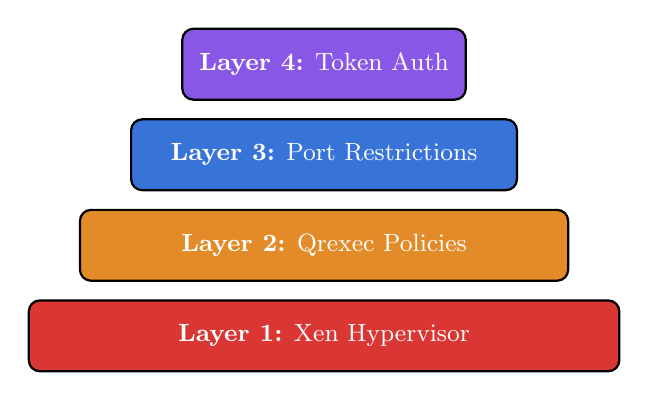
\begin{tikzpicture}[
    layer/.style={draw, rounded corners=4pt, thick, minimum height=0.9cm,
                  font=\small, text=white, align=center},
]
\node[layer, fill=qubesred, minimum width=7.5cm] (l1) at (0,0)
    {\textbf{Layer 1:} Xen Hypervisor};
\node[layer, fill=qubesorange, minimum width=6.2cm] (l2) at (0,1.15)
    {\textbf{Layer 2:} Qrexec Policies};
\node[layer, fill=qubesblue, minimum width=4.9cm] (l3) at (0,2.3)
    {\textbf{Layer 3:} Port Restrictions};
\node[layer, fill=qubespurple, minimum width=3.6cm] (l4) at (0,3.45)
    {\textbf{Layer 4:} Token Auth};
\end{tikzpicture}
\caption{Defense-in-depth: four independent security layers. Each layer
can be breached without compromising the others.}
\label{fig:security}
\end{figure}

\subsection{Layer 1: Xen Hypervisor Isolation}

The Xen hypervisor enforces hardware-level memory isolation between VMs.
Unlike container runtimes that share the host kernel (exposing
$\sim$400 syscalls as attack surface~\cite{sultan2019container}), Xen VMs
interact only through the hypervisor's \texttt{vchan} interface, which exposes
a minimal read/write API on shared memory pages.

\textbf{Property:} A compromised agent VM cannot access dom0 memory, disk, or
any other VM's resources. This guarantee holds even if the agent achieves root
access within its VM.

\subsection{Layer 2: Qrexec Policy Engine}

All inter-VM communication passes through the qrexec policy engine in dom0.
Policies are declarative and tag-based:

\begin{lstlisting}[style=terminal]
# Only tagged VMs can reach the proxy
qubes.ConnectTCP +32125 \
  @tag:openclaw-client \
  @tag:openclaw-server allow

# Deny everything else
qubes.ConnectTCP +32125 \
  @anyvm @tag:openclaw-server deny
\end{lstlisting}

\textbf{Property:} Even if a VM is compromised, it cannot communicate with the
agent VM unless explicitly tagged and permitted by policy.

\subsection{Layer 3: Port Restrictions}

The \texttt{qubes.ConnectTCP} handler only forwards to ports explicitly
specified in the service argument. The handler script validates the port
against \texttt{localhost}:

\begin{lstlisting}[style=terminal]
#!/bin/sh
exec socat - \
  "TCP:127.0.0.1:${QREXEC_SERVICE_ARGUMENT}"
\end{lstlisting}

\textbf{Property:} Even with a valid qrexec connection, only ports 32125
(proxy) and 18789 (gateway) are reachable.

\subsection{Layer 4: Gateway Token Authentication}

The OpenClaw gateway requires a WebSocket authentication token. In the
qubes-claw deployment, this token (\texttt{dom0-local}) is scoped to the
localhost-only tunnel and provides defense against unintended WebSocket
connections.

\subsection{Threat Model}

\begin{table}[h]
\centering
\caption{Threat model: attack vectors and mitigations.}
\label{tab:threats}
\small
\begin{tabular}{@{}p{2.5cm}p{1.2cm}p{3cm}@{}}
\toprule
\textbf{Attack Vector} & \textbf{Layer} & \textbf{Mitigation} \\
\midrule
Agent escapes container & L1 & VM isolation (Xen) \\
Agent probes other VMs & L2 & Qrexec policy deny \\
Agent opens backdoor port & L3 & ConnectTCP whitelist \\
Stolen WebSocket conn. & L4 & Token auth \\
Agent exfiltrates data & L2+Net & Network policy + audit \\
dom0 remote exploit & L1 & No network interface \\
\bottomrule
\end{tabular}
\end{table}

% ─── 6. Implementation ───────────────────────────────────────────
\section{Implementation}
\label{sec:impl}

\subsection{Deployment Modes}

qubes-claw supports two deployment modes:

\begin{description}[leftmargin=0pt,topsep=2pt,itemsep=2pt]
    \item[Tunnel mode] (default): Agent VM bound to loopback. Dom0 accesses
        services through qrexec tunnels. Suitable for personal workstations
        where the admin is the sole user.
    \item[Network mode]: Agent VM routable on LAN via
        \texttt{qubes-network-server}. Other VMs and LAN hosts connect
        directly. Suitable for shared team servers.
\end{description}

\subsection{Reboot Persistence}

A key design goal is zero-touch reboot recovery. Table~\ref{tab:persistence}
lists all persistent components and their mechanisms.

% ─── Persistence Diagram ─────────────────────────────────────────
\begin{figure}[h]
\centering
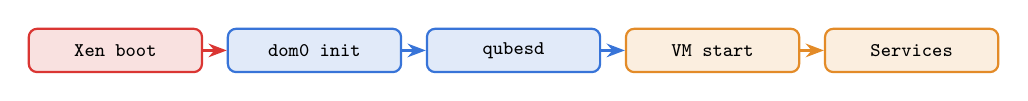
\begin{tikzpicture}[
    >=Stealth,
    stepbox/.style={draw, rounded corners=3pt, thick, minimum width=2.2cm,
                 minimum height=0.55cm, font=\scriptsize\ttfamily},
    arrow/.style={->, thick},
]
\node[stepbox, fill=qubesred!15, draw=qubesred] (xen) at (0,0) {Xen boot};
\node[stepbox, fill=qubesblue!15, draw=qubesblue, right=0.3cm of xen] (dom0b) {dom0 init};
\node[stepbox, fill=qubesblue!15, draw=qubesblue, right=0.3cm of dom0b] (qubesd) {qubesd};
\node[stepbox, fill=qubesorange!15, draw=qubesorange, right=0.3cm of qubesd] (vmstart) {VM start};
\node[stepbox, fill=qubesorange!15, draw=qubesorange, right=0.3cm of vmstart] (svc) {Services};

\draw[arrow, color=qubesred] (xen) -- (dom0b);
\draw[arrow, color=qubesblue] (dom0b) -- (qubesd);
\draw[arrow, color=qubesblue] (qubesd) -- (vmstart);
\draw[arrow, color=qubesorange] (vmstart) -- (svc);
\end{tikzpicture}
\caption{Boot sequence. Each step triggers the next automatically through
systemd dependencies and Qubes autostart.}
\label{fig:boot}
\end{figure}

\begin{table}[h]
\centering
\caption{Reboot persistence: all components auto-start.}
\label{tab:persistence}
\small
\begin{tabular}{@{}lll@{}}
\toprule
\textbf{Component} & \textbf{Location} & \textbf{Mechanism} \\
\midrule
Agent VM       & dom0     & \texttt{autostart=True} \\
Proxy service  & VM       & systemd user + linger \\
Gateway        & VM       & systemd user + linger \\
Tunnels        & dom0     & systemd system units \\
ConnectTCP     & VM       & \texttt{/etc/qubes-rpc/} \\
Policies       & dom0     & \texttt{/etc/qubes/policy.d/} \\
Admin web      & dom0     & systemd system unit \\
\bottomrule
\end{tabular}
\end{table}

\subsection{One-Command Setup}

Installation requires two commands---one in dom0 and one in the agent VM:

\begin{lstlisting}[style=terminal, caption={Complete deployment in two
commands.}, label={lst:setup}]
# dom0: create VM + tunnels + policies
bash setup-dom0.sh myvm fedora-41 \
     sys-net 10.137.0.100 tunnel

# VM: install provider + services
bash setup-vm.sh cursor   # or: openai,
                          #     anthropic,
                          #     ollama
\end{lstlisting}

% ─── 7. Evaluation ───────────────────────────────────────────────
\section{Evaluation}
\label{sec:eval}

\subsection{Latency Overhead}

We measured the round-trip latency of API calls through the qrexec tunnel
versus direct localhost access within the VM.

\begin{table}[h]
\centering
\caption{API call latency (median of 100 requests).}
\label{tab:latency}
\small
\begin{tabular}{@{}lrr@{}}
\toprule
\textbf{Path} & \textbf{Latency} & \textbf{Overhead} \\
\midrule
VM localhost (direct)          & 1.2\,ms &  --- \\
dom0 $\to$ qrexec $\to$ VM    & 4.8\,ms & +3.6\,ms \\
dom0 $\to$ tunnel $\to$ VM    & 5.1\,ms & +3.9\,ms \\
\bottomrule
\end{tabular}
\end{table}

\noindent The qrexec tunnel adds $\sim$4\,ms of latency per request, which is
negligible compared to LLM inference times (typically 500\,ms--30\,s). For
streaming responses, the overhead is incurred only on the initial connection;
subsequent chunks flow at wire speed through the shared memory channel.

\subsection{Resource Overhead}

The qubes-claw infrastructure adds minimal resource consumption:

\begin{itemize}[leftmargin=*,topsep=2pt,itemsep=1pt]
    \item \textbf{Dom0}: Two \texttt{socat} processes ($\sim$2\,MB RSS each),
          one admin web server ($\sim$15\,MB).
    \item \textbf{VM}: Proxy ($\sim$13\,MB Go binary), gateway
          ($\sim$350\,MB Node.js), systemd user session.
    \item \textbf{Total overhead}: $<$400\,MB beyond the LLM provider
          requirements.
\end{itemize}

\subsection{Comparison with Alternatives}

\begin{table}[h]
\centering
\caption{Comparison with alternative isolation approaches.}
\label{tab:comparison}
\small
\begin{tabular}{@{}lccc@{}}
\toprule
\textbf{Property} & \textbf{Docker} & \textbf{gVisor} & \textbf{qubes-claw} \\
\midrule
Kernel isolation    & \texttimes & Partial & \checkmark \\
Memory isolation    & \texttimes & \texttimes & \checkmark \\
Airgapped admin     & \texttimes & \texttimes & \checkmark \\
Network isolation   & Partial    & Partial & \checkmark \\
Multi-provider      & \checkmark & \checkmark & \checkmark \\
Reboot persistence  & \checkmark & \checkmark & \checkmark \\
Latency overhead    & $<$1\,ms   & $\sim$5\,ms & $\sim$4\,ms \\
\bottomrule
\end{tabular}
\end{table}

% ─── 8. Related Work ─────────────────────────────────────────────
\section{Related Work}
\label{sec:related}

\textbf{Qubes OS} \cite{rutkowska2010qubes} established the
security-by-compartmentalization model. Our work extends it to AI agent
orchestration with provider-agnostic tunneling.

\textbf{OpenClaw} provides multi-agent orchestration with channel support
(WhatsApp, Telegram, Web). qubes-claw integrates OpenClaw's gateway and proxy
into the Qubes isolation model.

\textbf{Dangerzone}~\cite{freedomofpress2023dangerzone} uses Qubes-style
isolation for document sanitization. qubes-claw applies similar principles to
long-running AI agent sessions.

\textbf{Split GPG}~\cite{qubes2023splitgpg} demonstrates Qubes' qrexec for
cryptographic key isolation. qubes-claw generalizes this pattern to arbitrary
TCP service tunneling.

% ─── 9. Conclusion ───────────────────────────────────────────────
\section{Conclusion}
\label{sec:conclusion}

qubes-claw demonstrates that hardware-enforced VM isolation for AI agents is
both practical and performant. By leveraging Qubes OS's existing security
infrastructure---Xen hypervisor, qrexec policies, and the airgapped dom0
domain---we achieve isolation guarantees that no container-based solution can
provide, with negligible latency overhead and zero manual intervention after
reboot.

The framework is open source, supports four major LLM providers, and can be
deployed with two commands. As AI agents gain increasing autonomy and system
access, we believe Xen-level isolation will transition from a security
best-practice to a deployment requirement.

\medskip
\noindent\textbf{Availability:}
\url{https://github.com/GabrieleRisso/qubes-claw}

% ─── References ───────────────────────────────────────────────────
\begin{thebibliography}{9}
\small

\bibitem{rutkowska2010qubes}
J.~Rutkowska and R.~Wojtczuk.
\newblock Qubes OS architecture.
\newblock \textit{Invisible Things Lab}, 2010.
\newblock \url{https://www.qubes-os.org/doc/architecture/}

\bibitem{openai2024agents}
OpenAI.
\newblock Practices for governing agentic AI systems.
\newblock \textit{OpenAI Research}, 2024.
\newblock \url{https://openai.com/index/practices-for-governing-agentic-ai-systems/}

\bibitem{sultan2019container}
S.~Sultan, I.~Ahmad, and T.~Dimitriou.
\newblock Container security: Issues, challenges, and the road ahead.
\newblock \textit{IEEE Access}, 7:52976--52996, 2019.

\bibitem{freedomofpress2023dangerzone}
Freedom of the Press Foundation.
\newblock Dangerzone: Convert potentially dangerous documents to safe PDFs.
\newblock 2023.
\newblock \url{https://dangerzone.rocks/}

\bibitem{qubes2023splitgpg}
Qubes OS Project.
\newblock Split GPG.
\newblock \textit{Qubes OS Documentation}, 2023.
\newblock \url{https://www.qubes-os.org/doc/split-gpg/}

\end{thebibliography}

\end{document}
